\documentclass[12pt, oneside,a4paper]{article}
\usepackage[latin1]{inputenc}
\usepackage{TW_corp_ID}
\definecolor{grau2}{gray}{0.95}

\usepackage{bibgerm}
\bibliographystyle{geralpha}

\usepackage{listings}
\renewcommand\lstlistingname{Listing}
\renewcommand\lstlistlistingname{Listings}
\lstdefinestyle{example} { %code listings: beispiele
		%language=Python,
    numbers=left, numberstyle=\scriptsize, stepnumber=1, numbersep=8pt,
    basicstyle=\ttfamily\footnotesize,
		backgroundcolor=\color{grau2},
		captionpos=b,
		showstringspaces=false,
		tabsize=4
		%commentstyle=\color{blue},%  Kommentar blau
		%keywordstyle=\color{red},%   Schl�sselw�rter rot
		%stringstyle=\color{green} % typewriter type for strings
}
\lstdefinestyle{interpreter} {%inline interpreter beispiele
		numbers=none,
		tabsize=4,
		basicstyle=\ttfamily\footnotesize,
		moredelim=[l][{\bfseries}]{>>>},
		moredelim=[l][{\bfseries}]{...}
}

% sollte als letztes Packet geladen werden (wenn glossary nicht verwendet wird ;) )
\usepackage{hyperref} 

\begin{document}
\pagestyle{TWcorpID}

\pagenumbering{arabic}

\section*{Kurzfassung: "'Python und Zope als Unterrichtswerkzeuge"'}
\rkopf[]{Bewerbung OCG F�rderpreis FH 2008 - Dominique Lederer}

	%Was will diese Arbeit? Warum wird sie geschrieben? Was ist das Ziel? Was ist der Mehrwert?
%Thema? Ziel?

Geht es um das Aneignen von Programmierkenntnissen, ist die momentane Situation nach Ansicht des Autors nicht optimal.
Sie ist verbesserungsw�rdig. Gerade in der schnelllebigen Informatik sollte im Unterricht nicht auf Trends oder Modeerscheinungen zur�ckgegriffen werden, sondern die fundamentalen Ideen der Wissenschaft Informatik mit einem guten Konzept an die Studierenden herangetragen werden. Erste Programmierkenntnisse mit z.B. C oder Java zu vermitteln bzw. vermittelt zu bekommen, ist problematisch. Diese Arbeit hat zum Ziel, einen einfacheren Weg aufzeigen und soll begr�nden, warum erste Programmiererfahrungen mit Python didaktisch sinnvoller sind.

Die Programmiersprache Python soll als Programmiersprache f�r den Unterrichtseinsatz vorgestellt werden und es wird gezeigt, wie gewisse Grundkonzepte mittels dieses Werkzeugs vermittelt werden k�nnen. Weiterf�hrend wird \Zope\ als Applikationsserver, basierend auf Python, f�r fortgeschrittenere Themen der Softwareentwicklung, und vor allem f�r den praktischen Teil dieser Arbeit verwendet.

Die Arbeit hat das Ziel, die Verbreitung von Python an Schulen und Universit�ten zu unterst�tzen, um damit den Sch�lern\footnote{Wenn in dieser Arbeit die m�nnliche Form verwendet wird, sind Frauen gleicherma�en gemeint, sofern nicht explizit Gegenteiliges behauptet wird.} und Studenten den Einstieg in die Programmierung und diese selbst zu erleichtern. 

Weiters ist \Zope\ f�r den Einsatz an Universit�ten vorzustellen; der einfache Zugang zu einem Open-Source Produkt soll die Vorteile f�r Lektoren und Studenten bei fortgeschrittenen Themen der Softwareentwicklung aufzeigen.

Die vorliegende Arbeit soll dabei als Entscheidungs- und Argumentationsgrundlage an genannten Ausbildungseinrichtungen dienen k�nnen.

%It has always been Van Rossum's desire to see Python used for teaching, 
 




	\section{Fundamentale Ideen als Unterrichtsprinzip}
	%Einleitende Worte zum Thema "Didaktisches Prinzip".\cite{bruner}
Eine Argumentationsgrundlage dieser Arbeit ist die Definition einer \emph{fundamentalen Idee} nach Schwill \cite{schwill1}. In seiner Arbeit untersucht er die philosophische Sicht der \emph{Idee} nach Plato und Kant, und formuliert diese mit den \emph{Strukturen} nach J.S. Bruner \cite{bruner} zur fundamentalen Idee. J.S. Bruner hat das didaktische Prinzip an den Strukturen der zugrundeliegenden Wissenschaft, an denen sich der Unterricht orientieren soll, formuliert.

\begin{quote}   
{\itshape "'Eine \textbf{fundamentale Idee} (bezgl. einer Wissenschaft) ist ein Denk-, Handlungs-, Beschreibungs- oder Erkl�rungsschema, das
\begin{enumerate}
	\item in verschiedenen Bereichen (der Wissenschaft) vielf�ltig anwendbar oder erkennbar ist (Horizontalkriterium),
	\item auf jedem intellektuellen Niveau aufgezeigt und vermittelt werden kann (Vertikalkriterium),
  \item in der historischen Entwicklung (der Wissenschaft) deutlich wahrnehmbar ist und l�ngerfristig relevant bleibt (Zeitkriterium),
  \item einen Bezug zu Sprache und Denken des Alltags und der Lebenswelt besitzt (Sinnkriterium)."'
\end{enumerate}}
\end{quote}

\begin{figure}[h]
	\centering
	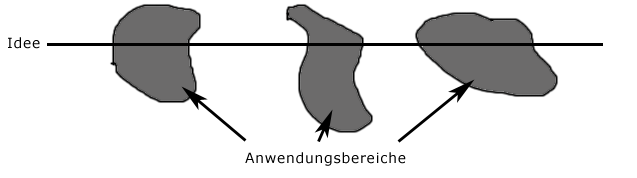
\includegraphics[scale=0.6]{graphics/horizontalkriterium.png}
	\caption{Horizontalkriterium nach \cite{schwill1}}
	\label{fig:horizontalkriterium}
\end{figure}

Das \emph{Horizontalkriterium} veranschaulicht Schwill wie in Abbildung \ref{fig:horizontalkriterium}. Eine Idee wird soweit abstrahiert, dass fachspezifische Elemente herausfallen. Damit kann themen- und fach�bergreifend gearbeitet werden. Der Lernende erkennt durch immer wiederkehrende Prinzipien die �bergreifende Relevanz der Thematik. Anschlie�end wird durch Wiederholung das Wichtige gefestigt. Die gemeinsame Idee kann jedoch wiederum nur durch umfassendes Spezialwissen herausgearbeitet werden. Das ist die Aufgabe der Lehrkr�fte.

Das \emph{Vertikalkriterium} kann wie ein Faden im Bildungsweg gesehen werden. Diesem Faden wird im Laufe der Ausbildung gefolgt. Dabei steigen das Niveau und die Detaillierung der Materie (Abbildung \ref{fig:vertikalkriterium}).

\begin{figure}[h]
	\centering
	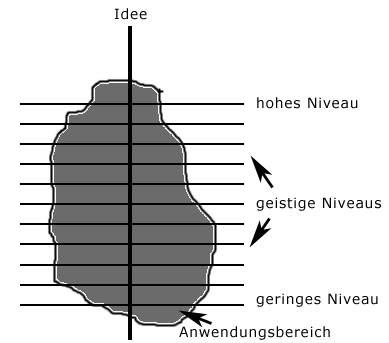
\includegraphics[scale=0.6]{graphics/vertikalkriterium.png}
	\caption{Vertikalkriterium nach \cite{schwill1}}
	\label{fig:vertikalkriterium}
\end{figure}

Das \emph{Zeitkriterium} ist in der Informatik nicht schwer zu erf�llen. Die Schnelllebigkeit der Technik birgt zwar viele Modeerscheinungen, jedoch sichert das Kriterium die Kontinuit�t des Unterrichts und den Wert der Kenntnisse und Erfahrungen der Unterrichtenden und verhindert fachliche Moden.\cite{misc:Modrow}

%\begin{quote}   
%{\itshape "'Das Kriterium sichert die Kontinuit�t des Unterrichts und den Wert der Kenntnisse und Erfahrungen der %Unterrichtenden und verhindert fachliche Moden."'}\cite{misc:Modrow}
%\end{quote}

Dabei ist die Tr�gheit der Lehre eine Art Vorauslese, um das Zeitkriterium einer fundamentalen Idee zu erf�llen.

Der Autor interpretiert das \emph{Sinnkriterium} als das tats�chliche Wertempfinden beim Empf�nger der Idee, beim Lernenden. Wie gut kann die Thematik als praxisrelevant oder als sinnvoll erkannt werden? Kann der Bezug zur sp�teren Verwendung in der Arbeitswelt hergestellt werden?

Der Einsatz fundamentaler Ideen wird von \cite{misc:Modrow} wie folgt beschrieben:

\begin{quote}   
{\itshape "'Der Unterricht muss dann so angelegt werden, dass sich diese - wenigen - fundamentalen Ideen bei den Sch�lerinnen und Sch�lern bilden k�nnen, er muss Kenntnisse und Erfahrungen vermitteln, die anhand dieser Ideen zu ordnen sind, und er muss diese Ideen zu einem geeigneten Zeitpunkt explizit thematisieren, um die spezifischen M�glichkeiten und Beschr�nkungen der Informatik in Abgrenzung gegen andere Disziplinen erkennbar zu machen."'}
\end{quote}

Einige Beispiele fundamentaler Ideen und die dazugeh�rigen Kriterien sind in \cite{schwill2} zu finden.

	\section{Programmiersprachen im Unterricht}
	\label{kapitel:Programmiersprachen}
	Ein vieldiskutiertes Thema ist, welche Sprache sich f�r den Unterricht am besten eignet. \cite{python:CRPITV52P71-80, misc:palumbo} meint, dass der Lernerfolg von der Zeit abh�ngt, die f�r tats�chliches Programmieren aufgewendet werden kann. Es sollte keine Zeit mit sprachspezifischen Eigenheiten und Syntaxproblemen "'verschwendet"' werden. Geht es nach \cite{python:CRPITV52P71-80, misc:milbrandt}, hat eine Programmiersprache f�r Unterrichtszwecke einen einfachen Zugang. Sie sollte leicht erlernbar sein, eine klare Struktur haben und vielf�ltig einsetzbar sein. Die Sprache hat eine einfache Syntax, einfaches I/O Handling, verst�ndliche String-Manipulation, aussagekr�ftige Schl�sselw�rter und verst�ndliches Feedback im Fehlerfall.

W�hrend Pascal und Logo vor einigen Jahren noch oft im Unterricht zum Einsatz kamen, sind beide heute stark aus der Mode gekommen. Gr�nde daf�r sind sicher die mangelnde Einsatzf�higkeit in der Industrie und die, so gut wie nicht m�gliche, Verwendbarkeit der Sprache bei steigender Komplexit�t der Software.

Heute z�hlen Sprachen wie C, Java und C++ zu den beliebtesten Programmiersprachen. Das ist an der Anzahl der verf�gbaren Entwickler, Lehrg�nge und Dienstleister weltweit zu erkennen \cite{misc:TIOBE}. Studien wie \cite{misc:deRaadt}, \cite{python:industry2} und \cite{misc:stephenson} belegen, dass Java, C++ und C die Sprachen mit der gr��ten Verbreitung an Universit�ten sind.

Trotz dieser Beliebtheit (oder gerade deswegen) wird viel �ber die Tauglichkeit dieser Sprachen im Unterricht diskutiert, gerade wenn es um geeignete Sprachen f�r Programmieranf�nger geht. Die oben genannten Sprachen werden als �berladen betrachtet. Die Studierenden plagen sich eher mit der Notation, als mit dem tats�chlichen Algorithmen. \cite{python:CRPITV52P71-80} erl�utert, dass die meisten Probleme von Programmierneulingen immer dasselbe Muster zeigen:
\begin{quote}
{\itshape "'[...] construct-based problems, which make it difficult to learn the correct semantics of language constructs, and plan composition problems, which make it difficult to put plans together correctly [...] students lack the skills needed to trace the execution of short pieces of code after taken their first course on programming."'}
\end{quote}

Im Zuge einer Studie an der finnischen Universit�t in Tampere ist eine Umfrage an europ�ischen Hochschulen durchgef�hrt worden. 559 Studenten und 34 Lektoren an 6 verschiedenen Universit�ten wurden unter anderem zu deren Schwierigkeiten beim Lernen und Lehren von Programmiersprachen befragt. Die daraus abgeleiteten Folgerungen besagen:
\begin{quote}
{\itshape "'the most difficult concepts to learn are the ones that require
understanding larger entities of the program instead of just details [...] abstract concepts like pointers and memory handling are difficult
to learn [...] However, the biggest problem of novice programmers does not seem to be the understanding of basic concepts but rather learning
to apply them."'}\cite{misc:difficulties}
\end{quote}

Die Studenten haben Probleme, wenn es darum geht, den Gesamtumfang eines Programmes zu erfassen und umzusetzen, dh. wie setze ich eine mir gestellte Aufgabe mit den Konzepten um, die ich gelernt habe. Dabei darf die Syntax einer Sprache nicht im Wege stehen, da sie daran hindert eine Probleml�sung zu finden und nur neue, andere Probleme schafft. Zeiger und Speichermanipulation z�hlen zu den als sehr schwierig eingestuften Konzepten.

Die in diesem Kapitel zitierte Literatur deckt sich mit den Beobachtungen des Autors aus der eigenen Ausbildung und der Abhaltung eines C Tutoriums f�r Programmieranf�nger. Die Studenten konnten genau wiedergeben, wie sie das Problem l�sen w�rden, doch konnten sie es nicht "'zu Papier"' bringen, also als Quelltext wiedergeben. Die Syntax wurde als unnat�rlich und teilweise unverst�ndlich empfunden. Manche syntaktische Eigenheiten sind f�r den Tutor auch schwer zu erkl�ren, da die Studenten die dahinterliegenden Konzepte noch nicht verstehen k�nnen. Nahezu alle Fehler resultierten aus einem Fehler in der Syntax. Der Autor konnte dabei ein hohes Ma� an Frustration und Demotivation der Studenten im Unterricht feststellen. Die Sinnhaftigkeit des Lehrinhaltes wurde weiters angezweifelt.
	
	\section{Python als erste Programmiersprache?}
	\label{sec:firstlanguage}
	Warum eignet sich Python als Werkzeug f�r den Informatikunterricht? Ist Python als Einstiegssprache geeignet? Was zeichnet Python gegen�ber anderen Programmiersprachen aus? Welche Anforderungen werden an eine "'erste Programmiersprache"' gestellt? Was haben die Lehrenden davon? Dieses Kapitel enth�lt eine Diskussion zu den vorangegangen Fragen. 

Gegenw�rtig sind haupts�chlich Java und C++ als Programmierprachen in Lehrg�ngen f�r Programmieranf�nger anzutreffen (vgl. Kapitel \ref{kapitel:Programmiersprachen}) \cite{python:firstlanguage6}.

\begin{quote}
{\itshape "'While students with good preliminary background, who have already committed themselves to a computing career, usually succeed in such courses, many others remain disappointed or even completely fail."'}
\end{quote}

\cite{python:firstlanguage6} schreibt, dass Studenten mit Vorkenntnissen und explizitem Interesse an der Materie es leichter haben, solche Kurse erfolgreich zu absolvieren. Studenten, die bisher keine Erfahrungen in der Programmierung haben, bleiben hier oft auf der Strecke. Die Motivation, die Materie weiter zu verfolgen, ist verst�ndlicherweise gering. Dabei soll Unterricht �blicherweise motivieren und dadurch den Forschergeist wecken. Ob das gelingt, ist eine Frage der Gestaltung des Unterrichts und h�ngt nur geringf�gig von der zu unterichtenden Materie ab. Jedes noch so trockene Thema kann durch interessante und fesselnde Unterrichtsgestaltung schmackhaft gemacht werden. Die Unterrichtsgestaltung h�ngt auch mit der Wahl der benutzten Werkzeuge, um Wissen zu vermitteln, zusammen.

Das Problem nach \cite{python:firstlanguage6} ist, dass die heute verwendeten Sprachen alle kommerziell ausgerichtet sind. Kommerzielle Sprachen sind nicht f�r den Unterricht ausgelegt, sondern f�r die industrielle Softwareentwicklung. Kommerzielle Applikationen sind komplex. Die Programmiersprachen sind daf�r ausgelegt, die Entwicklung dieser Applikationen zu erm�glichen.

Der Autor unterst�tzt diese Argumentation. Es stellt sich jedoch die Frage, warum nicht gerade aus diesen Gr�nden Programmiersprachen so einfach und �bersichtlich wie m�glich sein sollten. Eine Ursache daf�r ist sicher eine versuchte Effizienzsteigerung durch diverse Sprachkonstrukte, die den Profi effizienter arbeiten lassen, f�r Anf�nger aber nicht leicht verst�ndlich sind ("make the common case efficient"). \cite{python:firstlanguage6} meint in seiner Arbeit, dass genau aus diesem Grund Programmierneulinge mit Konzepten konfrontiert werden, die f�r den Anfang �berfordern.

\cite{python:firstlanguage1} bringen einen Vergleich f�r den sportlichen Leser, indem sie ein Beispiel aus dem Schifahren bringen. Um ein wirklich guter Schifahrer zu werden, erfordert es �bung. Schipisten sind darauf ausgelegt, das �ben zu unterst�tzen, indem sie je nach Schwierigkeitsgrad farblich markiert sind. Blau f�r Anf�nger, Rot f�r Fortgeschrittene und Schwarz f�r Profis. Eine blaue Piste bedeutet aber nicht, das hier auf die wichtigen Elemente des Schifahrens zu verzichten ist. Schw�nge, Geschwindigkeitskontrolle, Bremsen und die richtige �bersicht sind auch hier notwendig, sind jedoch unter entsch�rften Bedingungen aus�bbar. Wird ein Anf�nger auf die schwarze Piste geschickt, wird er oft st�rzen. Die Erfahrung ist f�r ihn frustrierend, und er wird schnell aufgeben und den Sport verdammen.

Dieser Ausflug in eine anderes Gebiet und die einfache Erkenntnis daraus kann auf jedes Lernen umgelegt werden. Konfrontiert man den Lernenden zu fr�h mit zu hoher Komplexit�t, kann dieser nicht genug Erfolge erleben und wird sich eher frustriert von der Thematik abwenden. Der Stoff muss sich aufbauend an den fundamentalen Ideen des Unterrichtsgegenstandes n�hern, und dem Lernenden zwischendurch immer wieder Erfolgserlebnisse erm�glichen.

\begin{quote}
{\itshape "'As students progress through the introductory computer science sequence, we want them to
focus on aspects of problem solving, algorithm development, and algorithm understanding.
Unfortunately, many modern programming languages require that students jump into more
advanced programming concepts at a point that is too soon in their development. This
sets them up for possible failure, not because of the computer science but because of the
language vehicle being used."'}\cite{python:firstlanguage1}
\end{quote}

In der Informatik liegt das Augenmerk auf den Aspekten der Probleml�sung, der Entwicklung und dem Verstehen von Algorithmen. Die heute im Unterricht angewandten Programmiersprachen f�hren aber zu fr�h in komplexere Details der Wissenschaft. Das f�hrt auch dazu, dass nicht Informatik, sondern die Aspekte einer Programmiersprache zum Gegenstand des Unterichts werden.

\begin{quote}
{\itshape "'It is a shame that the languages that our students encounter when they come to learn to program are
languages that are designed for commercial use by experienced commercial programmers. Modern languages
like Java and C++ contain a host of features that most students will never need, and which we should
probably admit are a mystery to many of the students' teachers."'}\cite{python:firstlanguage2}
\end{quote}

Sprachen wie Java oder C++ sind in ihrem Umfang so m�chtig, das es bestimmt eher selten ist, wirklich routinierte Profis als Lektoren zu bekommen. Gl�cklich sind diejenigen, die in diesen Genuss kommen. 

\subsubsection*{Industriesprachen}

We�halb werden Java, C++ und C nun haupts�chlich verwendet? Geht es nach \cite{python:firstlanguage2}, \cite{python:CRPITV52P71-80}, \cite{python:firstlanguage7}, \cite{python:industry1}, \cite{python:industry2} und \cite{python:firstlanguage9}, ist dieser Zustand industriegetrieben. Studenten sehen Jobangebote, in denen eine bestimmte Programmiersprache als Voraussetzung verlangt wird, und wollen diese lernen, um ihre Qualifikation damit aufzuwerten. Sie haben kein Interesse, eine "'Baby-Sprache"'\cite{python:firstlanguage11} zu lernen. Lehreinrichtungen bewerten ihre Studienpl�ne anhand der Nachfrage in der Industrie. Das betrifft ganz besonders Fachhochschulen, wo Lehrpl�ne in enger Zusammenarbeit mit der Industrie erstellt werden. 

Ein Lektor des Autors, der lieber anonym bleiben m�chte, ist da ganz anderer Meinung. Die obig gebrachten �berlegungen seien unwahr, vielmehr gestaltet sich der Unterricht oft nach der Verf�gbarkeit von Lektoren im Bekanntenkreis der f�r den Studienplan verantwortlichen Personen. Diese Lektoren bringen eher ihre pers�nlich bevorzugten Themen und Werkzeuge in den Unterricht ein (wobei letzteres durchaus legitim und wichtig f�r die Qualit�t des gebrachten Unterichtsstoffes ist).

Nach Ansicht des Autors ist die Realit�t wohl eine Mischung aus beiden gerade genannten Punkten. Doch sollte es nicht anders sein? In der Informatik war es fr�her auch anders. Blickt man auf die Zeit vor der objektorientierten Bewegung zur�ck, gab es Pascal \cite{misc:pascal} als allgemein anerkannte Programmiersprache f�r den Unterricht \cite{python:firstlanguage6},\cite{python:firstlanguage7}. Das Problem mit reinen Unterrichtssprachen wie Pascal  ist jedoch, dass sie in der Industrie nicht verwendet werden. Aus diesem Grund wurde Pascal auch weltweit aus den Lehrpl�nen gestrichen. 

Es braucht also eine Sprache, die
\begin{itemize}
	\item in der Industrie anerkannt ist bzw. in der Industrie Verwendung findet,
	\item mit der komplexe Softwareprojekte umgesetzt werden k�nnen,
	\item die f�r den Unterrichtseinsatz geeignet ist.
\end{itemize}

Betrachten wir Python, sind die ersten beiden Punkte erf�llt. Wenden wir uns nun dem dritten Punkt zu. Ist Python f�r den Unterrichtseinsatz geeignet?

\subsubsection*{Hello World}

\emph{Hello World} ist traditionellerweise das erste Programm jedes Programmieranf�ngers. Starten wir gleich mit der Python Variante.

\begin{lstlisting}[style=example, caption={Hello World mit Python}, label=python:helloworldpython]
print "Hello World!"
\end{lstlisting}

Nun zur C++ Variante des Programms.

\begin{lstlisting}[style=example, caption={Hello World mit C++}, label=python:helloworldC++]
#include <iostream>

using namespace std;

int main ()
{
  cout << "Hello World!";
  return 0;
}
\end{lstlisting}

\begin{itemize}
	\item Zeile 1: Zeilen, die mit einer Raute(\#) beginnen, sind Direktiven f�r den Pr�prozessor. Diese Zeilen werden vom Compiler nicht normal ausgewertet, sondern zuvor vom Pr�prozessor bearbeitet. Dieser reagiert je nach Befehl unterschiedlich. In diesem Beispiel wird dem Pr�prozessor mitgeteilt, die Datei \verb|iostream| zu inkludieren. Diese enth�lt Deklarationen der Standard Eingabe-Ausgabe Bibliothek von C++. Sie wird ben�tigt, da wir einen Befehl aus dieser Bibliothek sp�ter im Programm verwenden.
	\item Zeile 3: Alle Elemente der Standard C++ Bibliothek werden in einem eigenen Namensraum deklariert. Dieser Namensraum hat den Namen \verb|std|.
	\item Zeile 5: Die \verb|main| Funktion ist der Startpunkt eines jeden C++ Programmes. Eine Funktion wird immer mit runden Klammern definiert. Innerhalb der runden Klammern k�nnen Parameter an die Funktion �bergeben werden. Die geschwungenen Klammern markieren den Bereich der Funktion. Alles innerhalb dieser Klammer wird beim Aufruf der Funktion ausgef�hrt. Vor dem Namen der Funktion steht die Definition des R�ckgabewertes.
	\item Zeile 7: Das ist ein C++ Befehl (statement), den wir �ber eine Library inkludiert haben und einem Namesraum zugewiesen haben. Dieser spezielle Befehl repr�sentiert den \emph{Standard Output Stream} in C++. Das Beispiel zeigt, wie eine Sequenz von Zeichen ("'Hello World!"') in den Stream geschrieben wird. Jeder Befehl muss mit einem Semikolon (;) beendet werden.
	\item Zeile 8: Der \verb|return| Befehl beendet die Funktion, der Returnwert muss vom gleichen Typ wie die Deklaration der Funktion sein. Der Returncode von 0 bedeutet, das die Funktion fehlerfrei ausgef�hrt wurde.
\end{itemize}

Wie zu sehen ist, m�ssen, bei diesem sehr simplen Beispiel, Themen, die f�r einen Anf�nger doch sehr fortgeschritten sind, erl�utert werden. Eine andere, und nach Erfahrung des Autors sehr beliebte Variante um diese Problematik zu umschiffen, ist das gezielte Ignorieren dieser Punkte. Der Vortragende ersucht die Studenten, gewisse Teile des Programmes einfach auszublenden und z.B. nur innerhalb der \verb|main| Funktion zu arbeiten und zu denken.

\begin{quote}
{\itshape "'The C++ version has always forced me to choose between two unsatisfying options: either to explain the \#include,   void main(), \{, and \} statements, and risk confusing or intimidating some of the students right at the start, or to tell them 'just don't worry about all of that stuff now, we will talk about it later' and risk the same thing."'}\cite{python:firstlanguage10}
\end{quote}

Keine der beiden Varianten ist befriedigend. \cite{python:firstlanguage10} beschreibt den Aufwand, ein \emph{Hello World} Programm in ein Skriptum zu verfassen, wie folgt.

\begin{quote}
{\itshape "'There are thirteen paragraphs of explanation of "'Hello, world"' in the C++ version, in the Python version there are only three. More importantly, the missing ten paragraphs do not deal with the "'big ideas"' in computer programming, but with the minutia of C++ syntax. I found this same thing happening throughout the chapters that I have completed so far. Whole paragraphs simply disappear from the Python version of the text because Python's much simpler syntax renders them unnecessary."'}
\end{quote}

\cite{python:firstlanguage10} zeigt damit, dass viel Einf�hrungsarbeit mit C++ auf Spracheigenheiten bezogen ist. Das ist Zeitverschwendung. Studenten k�nnten mit Python viel fr�her zu ersten Erfolgserlebnissen kommen, ohne �ber mysteri�se Gegebenheiten, wie unerkl�rte und nicht verstandene Konstrukte, in den eigenen Programmen zu stolpern.

Bei der Java Version des Programmes wird der Student sofort mit einem fortgeschrittenen Konzept konfrontiert, welches aber das Wissen �ber darunterliegende, objektorientierte Thematik  voraussetzt. 

Der Autor will C++ und Java nicht negativ darstellen. Es soll lediglich aufgezeigt werden, dass ein Start in die Programmierung mit einer der momentan in der Ausbildung verwendeten Sprachen nicht als optimal angesehen werden kann. Ein gro�er Vorteil von Python im Vergleich der \emph{Hello World} Programme, ist die unterschiedliche Anzahl der Konzepte, die verstanden werden m�ssen, um ein erstes Programm zu schreiben. Ein erstes funktionales Programm ist auch ein erstes Erfolgserlebnis und motiviert zu mehr.

\subsubsection*{Syntax}

\begin{quote}
{\itshape "'Compared to languages such as Java or C++, Python has a more intuitive syntax. Python enforces an intended and structured way of writing programs, and the code resembles pseudo code."'}\cite{python:CRPITV52P71-80}
\end{quote}

Entwickler werden unter Python gezwungen, mit Einr�ckung ihres Quelltextes zu arbeiten. Eine Einr�ckung markiert einen Block im Programm. Der Block endet erst mit der Einr�ckung. Bei falscher Einr�ckung wird ein Fehler generiert. Dabei sieht ein Programm in Python fast genauso aus wie das Programm geschrieben in Pseudocode. Das hat den Vorteil, dass Algorithmen einfach nach Pseudocodevorlage implementiert werden k�nnen.

\begin{quote}
{\itshape "'[...] with Python, the Pseudocode is in fact also real code, and already executable."'}
\end{quote}

\cite{python:firstlanguage9} meint sogar, dass mit Python sei Pseudocode auch echter Quelltext, der schon ausf�hrbar ist.

Die Einr�ckung zwingt dazu, strukturiert zu schreiben und f�rdert dadurch ein einheitliches Programmbild, w�hrend in anderen Sprachen verschiedene Schreibstile m�glich sind, die dazu f�hren, dass Richtlinien zur Lesbarkeit entwickelt werden m�ssen.

Programme werden lesbarer, was einige Vorteile mit sich bringt. Lektoren haben es leichter, die Arbeit der Studenten zu evaluieren und finden auch schneller Fehler in Programmen. Da Python keine unterschiedlichen syntaktischen Stile erlaubt, ist es somit f�r Studenten einfacher, an gr��eren Projekten gemeinsam zu arbeiten.\cite{python:firstlanguage10}

\begin{quote}
{\itshape "'Novice programmers find indentation to be quite natural and we have found that it enforces a more readable coding
style than students typically adopt when they can use braces."'}\cite{python:firstlanguage1}
\end{quote}

Listing \ref{c:indent} zeigt ein C++ Beispiel. Frei nach dem Auge w�rde der zweite Befehl zum if-Block geh�ren. Durch das Fehlen der geschwungen Klammern umfasst der Block jedoch nur den ersten Befehl, der zweite wird unabh�ngig von der Verzweigung ausgef�hrt. Dieser Fehler passiert recht h�ufig. Mit Python w�re dieses Beispiel klar, alles Einger�ckte nach der Verzweigung ist dem Block zugeh�rig. Es herrscht eine Art "'nat�rliche Lesbarkeit"'.

\begin{lstlisting}[style=example, caption={Beispiel zur Lesbarkeit von einger�cktem Quelltext}, label=c:indent]
if(t == 1)
	cout << "t is 1";
	t = 2;
\end{lstlisting}

\begin{quote}
{\itshape "'We feel that writing structured programs, which are easy to check, follow and maintain, is one of the main lessons in any programming course. Using Python, this lesson is taught automatically."'}\cite{python:CRPITV52P71-80}
\end{quote}

Lesbaren Quelltext zu schreiben ist ein wichtiges didaktisches Ziel. Durch Python erreicht der Student das implizit.


\subsubsection*{Semantik}

Durch die dynamische Typisierung erspart man sich das Konzept der Deklaration. Der Typ einer Variable wird zur Laufzeit bestimmt. Eine Variable zeigt immer auf ein Objekt. Dieses Konzept ist leichter zu erl�utern und zu verstehen, als die maschinennahe statische Typisierung, wo eine Variable ein Platz im Speicher ist, der zuvor deklariert werden muss. Typisierung ist ebenfalls eine h�ufige Fehlerquelle, auf die anfangs getrost verzichtet werden kann. Auch Zeiger und Speicherverwaltung sind solche Konzepte.

Die Literatur ist sich einig, dass die genannten Konzepte f�r eine erste Programmiersprache nicht notwendig sind, aber trotzdem zu einem sp�teren Zeitpunkt gelehrt werden sollten. Erfahrungen zeigen, dass die Konzepte auch viel einfacher angenommen werden, nachdem Studenten ihre ersten Erfolge mit Python erlebt haben und in der Lage sind, eigene komplexe Programme zu schreiben. Der Umstieg auf eine Hochsprache ist unproblematisch.\cite{python:firstlanguage2, python:firstlanguage5, python:firstlanguage6, python:firstlanguage7, python:firstlanguage10, python:firstlanguage11}

\begin{quote}
{\itshape "'We believe that it is advantageous for beginning students to spend time on the green runs[blaue Piste] learning the rudimentary ideas relating to algorithms and data structures. If you are among those of our colleagues who are frustrated with Java or C++, we encourage you to consider Python and join us on the green runs, it works."'}
\end{quote}

\cite{python:firstlanguage10} nimmt wieder das Beispiel des Schifahrens als Illustration und vergleicht Python als erste Programmiersprache mit dem Fahren auf einer blauen Piste, wo Studenten, unter entsch�rften Bedingungen, das Arbeiten mit Algorithmen und Datenstrukturen lernen.
	
	\section{Programmierparadigmen im Unterricht}
	%TODO {\color{red} Paper download: http://ieeexplore.ieee.org/xpl/freeabs\_all.jsp?arnumber=839221, und http://portal.acm.org/citation.cfm?id=201998.202006}

Das Wort \textbf{Paradigma} kommt aus dem Griechischen und bedeutet Vorbild, Beispiel, Muster oder Abgrenzung. Es hat viele unterschiedliche Bedeutungen, die sich in der Wissenschaft, der Linguistik, Organisationstheorie etc. wiederfinden. F�r diese Arbeit und dieses Kapitel ist das Programmierparadigma interessant:

Ein \textbf{Programmierparadigma} ist das einer Programmiersprache oder Programmiertechnik zugrundeliegende Prinzip. Es ist eine Sichtweise, die zur L�sung eines Problems mittels einer Programmiersprache eingenommen wird.\cite{misc:multiparadigm}

Python ist prim�r eine objektortientierte Sprache, unterst�tzt also das objektorientierte Softwareparadigma:

\begin{quote}
{\itshape "'Python is a dynamic object-oriented programming language that can be used for many kinds of software development."'}\cite{python:website}
\end{quote}

Jedoch ist der Entwickler bei der Verwendung von Python an kein spezielles Paradigma gebunden. Python kann somit als \textbf{Multiparadigmen-Sprache} bezeichnet werden. 

In diesem Kapitel wird auf folgende Paradigmen kurz eingegangen und deren Realisierung mit Python erl�utert:

\begin{itemize}
	\item Imperative Programmierung
		\begin{itemize}
			\item Prozedurale Programmierung
			\item Modulare Programmierung
			\item Objektorientiere Programmierung
		\end{itemize}
	\item Deklarative Programmierung
		\begin{itemize}
			\item Funktionale Programmierung
  		\item Logische Programmierung
  	\end{itemize}
  \item Weitere Paradigmen
    \begin{itemize}
		  \item Design by Contract
		  \item Aspektorientierte Programmierung
		  %\item Komponentenortientierte Programmierung
    \end{itemize}
\end{itemize}

\subsubsection{Programmierparadigmen im Unterricht}

Nach \cite{misc:placer} und \cite{misc:westbrook} sind Multiparadigmensprachen f�r den Unterricht gut geeignet. Es ist wichtig den Studenten in kein Korsett hineinzuzwingen, sondern ein breites Schema an M�glichkeiten zur kreativen Entfaltung anzubieten, denn

\begin{quote}
{\itshape "'verschiedene Menschen nehmen zur L�sung von gleichen Aufgaben unterschiedliche Sichtweisen ein, und ebenso kann es sein, dass ein Mensch f�r unterschiedliche Aufgaben verschiedene L�sungsans�tze verfolgt. F�r die wenigsten Probleme gibt es die optimale L�sung, und so empfiehlt es sich, der- oder demjenigen, der das Problem l�st, die Wahl zu �berlassen, wie er oder sie am besten mit einer Aufgabe umgeht. Daher ist es f�r den praktischen
Einsatz von Programmiersprachen notwendig, diese unterschiedlichen Sichtweisen, die zu verschiedenen L�sungsstrategien f�hren, in geeigneter Form ausdr�cken zu k�nnen."'}\cite{misc:multiparadigm}
\end{quote}

Das bietet den Studenten den Freiraum, zu Beginn ihrer Programmierkarriere mittels \textbf{eines} Werkzeugs, n�mlich der Programmiersprache,  unterschiedliche Denkweisen und Programmierans�tze zu erproben. Die Studenten k�nnen sich voll und ganz auf das Verstehen der, den Paradigmen zugrundeliegenden Prinzipien konzentrieren und begreifen, dass ein Paradigma nicht von der verwendeten Programmiersprache abh�ngt, sondern von der Sichtweise auf eine Problemstellung und deren L�sung.

\begin{quote}
{\itshape "'Python erm�glicht sowohl den Logo-Zugang mit Rekursion und Listen, als auch den sequentiellen Zugang der imperativen Sprachen (und wer will - es geht auch funktional). Sprachen wie Delphi oder C++ zwingen den Sch�ler erst einmal, 'nur nichts falsch' zu machen. Das mag Sprach-Juristen erfreuen, l�sst aber den Forschungsdrang der Sch�ler verk�mmern."'}\cite{misc:urban}
\end{quote}

\subsubsection{Imperative Programmierung}

Imperative Programmierung ist das �lteste Programmierparadigma und ist an die Architektur 
des Von-Neumann-Rechners angelehnt. Ein Programm ist eine Folge von Anweisungen, die nacheinander abgearbeitet werden; dieses befindet sich zu jeder Zeit in einem Zustand, der vom Arbeitsspeicher und der Programmumgebung (Dateisystem, 
Peripherie) definiert ist. Seiteneffekte (Ein-/Ausgabe, Speichermodifikation, Variablen) bewirken 
eine �nderung des Zustandes �ber der Zeit.

\paragraph*{Prozedurale Programmierung}

Die prozedurale Programmierung, die als Synonym f�r imperative Programmierung gesehen werden kann,  
erm�glicht das Zusammenfassen von Anweisungen zu Unterprogrammen (Prozeduren). Unterprogramme
werden dann von verschiedenen Stellen des Programms aufgerufen und ausgef�hrt.

Das ist der erste Ansatz, Aufgaben in Teilaufgaben zu zerlegen und so eine einfachere, �bersichtlichere und vor allem wiederverwertbare Programmierung zu erm�glichen.

Es bietet sich an, dieses Paradigma als erstes im Unterricht vorzustellen, da Von-Neumann �blicherweise
sehr fr�h im Informatikunterricht ein Thema ist, und so ein einfacher Konnex hergestellt werden kann.

Um den zeitlichen Ablauf eines Programmes zu veranschaulichen, kann der Python Interpreter als 
unterst�tzendes Visualisierungswerkzeug im Unterricht verwendet werden:

\begin{lstlisting}[style=interpreter]
>>> fahr = 0
>>> while (fahr < 120):
...		celsius = 5./9 * (fahr - 32)
...		print 'Fahrenheit %6.1f = Celsius %6.3f' % (fahr, celsius)
...		fahr += 20
...
Fahrenheit    0.0 = Celsius -17.778
Fahrenheit   20.0 = Celsius -6.667
Fahrenheit   40.0 = Celsius  4.444
Fahrenheit   60.0 = Celsius 15.556
Fahrenheit   80.0 = Celsius 26.667
Fahrenheit  100.0 = Celsius 37.778
\end{lstlisting}

Die prozedurale Variante des obigen, sehr simplen, Beispiels erg�be dann mit ausgelagerter Berechnung:

\begin{lstlisting}[style=example, caption={Prozedurales Programmierbeispiel}, label=python:prozedural]
def fahr2cels(fahr):
	celsius = 5./9 * (fahr - 32) 
	print 'Fahrenheit %6.1f = Celsius %6.3f' % (fahr, celsius) 
	return celsius
  
fahr = 0
while (fahr < 120):
	fahr2cels(fahr)
	fahr += 20
\end{lstlisting}

\paragraph*{Modulare Programmierung}

Modulare Programmierung geht einen Schritt weiter und zerlegt die Prozeduren zusammen mit Daten in logische Einheiten: die Module. Der n�chste Schritt ist, Aufgaben in gr��eren Softwareprojekten zu abstrahieren. Die jeweiligen Module werden einzeln geplant, entwickelt und getestet.

Mit Python ist jede Datei ein eigenes Modul. Ein Verzeichnis mit Modulen wird Package\footnote{http://docs.python.org/tut/node8.html} genannt. Die Python Standardbibliothek und alle Erweiterungen werden als Packages entwickelt und eingebunden.

Wenn die Prozedur aus Listing \ref{python:prozedural} in eine eigene Datei names \verb|mymodule.py| ausgelagert wird, muss diese als Modul eingebunden werden:

\begin{lstlisting}[style=interpreter]
>>> from mymodule import fahr2cels
>>> fahr2cels(0)
Fahrenheit    0.0 = Celsius -17.778
\end{lstlisting}

Um das Modul nun f�r externe Pythonmodule zug�nglich zu machen, muss die Datei \verb|__init__.py| erstellt werden, die das Verzeichnis als Pythonpackage markiert.
Importiert wird das Modul auf unterschiedliche Arten. Dazu ein Beispiel:

\begin{lstlisting}[style=interpreter]
>>> from mydirectory.mymodule import fahr2cels
\end{lstlisting}

Das Kennenlernen der Modularisierung f�rdert das Verst�ndnis der Austauschbarkeit und Wiederverwendbarkeit von Software in einem sehr fr�hen Stadium des Unterrichts. Ohne viele Vorkenntnisse kann der Sinn und Zweck einer solchen Aufteilung erl�utert werden. Zu diesem Zweck k�nnten sich jeweils zwei Gruppen von Studenten zusammenfinden, die unterschiedliche Aufgaben zu l�sen haben. Die Aufgabe ist, ein Programm mittels eines weiteren Moduls zu entwerfen. Dieses Modul wird trotz unterschiedlicher Aufgabenstellung von beiden Studentengruppen ben�tigt. Interessant ist, die Studenten im ersten Anlauf unwissend in den Einzelgruppen arbeiten zu lassen. Danach werden die "Partnergruppen"' einander vermittelt und die jeweiligen, sicher unterschiedlich implementierten, L�sungen des Moduls von den Studenten zu einem gemeinsamen Modul angeglichen. Nat�rlich wird das nicht ganz friktionsfrei von statten gehen. Die �nderungen werden mit gro�er Wahrscheinlichkeit auch die beiden Programme der Gruppen betreffen.

Im zweiten Anlauf setzt man, mit neuer Aufgabenstellung,  die Studenten schon vorher �ber ihre jeweiligen Partner in Kenntnis. Nun soll ein gemeinsames Modul konzipiert werden, bevor man sich �ber die eigene Implementierung im Detail Gedanken macht. Die Schlu�folgerungen daraus werden anschlie�end diskutiert, die Studenten haben die ersten Untiefen der kollektiven Softwareentwicklung erlebt.

\paragraph*{Objektorientierte Programmierung}

Die \OOP\ erweitert das prozedurale Paradigma um Objekte. 

\begin{quote}
{\itshape "'Ein Objekt ist ein Gegenstand des Interesses, insbesondere einer Beobachtung, Untersuchung oder Messung. Objekte k�nnen Dinge, Personen, oder Begriffe sein [...] ein Objekt besitzt einen bestimmten Zustand und reagiert mit einem definierten Verhalten auf seine Umgebung [...] jedes Objekt besitzt eine Identit�t, die es von anderen Objekten unterscheidet [...] ein Objekt kann ein oder mehrere andere Objekte kennen."'}\cite{Balzert2004}
\end{quote}

Heide Balzert schreibt weiters, dass der Zustand eines Objektes dessen Attribute und die jeweiligen Verbindungen zu anderen Objekten umfasst. Das Verhalten eines Objektes wird durch die Menge seiner Operationen (Methoden, Funktionen) beschrieben. Eine �nderung oder eine Abfrage des Zustandes ist nur mittels Operationen m�glich (Geheimnisprinzip). Objekte werden durch Klassen definiert und k�nnen ihre Eigenschaften und Operationen vererben, was eine Schachtelung des Quelltextes erm�glicht.

Folgendes Listing zeigt eine typische Python Klasse:

\begin{lstlisting}[style=example, caption={einfache Python Klasse}]
class Bankkonto:

   def __init__(self,startbetrag):
      """Konstruktor"""
      self.kontostand = startbetrag

   def einzahlung(self, betrag):
      self.kontostand = self.kontostand + betrag

   def auszahlung(self, betrag):
      self.kontostand = self.kontostand - betrag

   def anzeigen(self):
      print self.kontostand
\end{lstlisting}

Wie zu Beginn dieses Kapitels erw�hnt, ist Python eine objektorientierte Programmiersprache. In Python ist alles ein Objekt, wie folgendes Beispiel zeigt.

\begin{lstlisting}[style=interpreter]
>>> konto = Bankkonto(100)
>>> Bankkonto
<class __main__.Bankkonto at 0x401dfbcc>
>>> konto
<__main__.Bankkonto instance at 0x401e972c>
>>> konto.anzeigen
<bound method Bankkonto.anzeigen of <__main__.Bankkonto instance at 0x401e972c>>
\end{lstlisting}
%TODO dieses listing l�sst kapitel Weitere Paradigmen rot erscheinen?

Python l�sst sich somit hervorragend f�r den aufbauenden Unterricht einsetzen. W�hrend mit Java ab dem ersten Programm der objektorientierte Ansatz verstanden werden muss, kann bei Python der Unterricht mit dem verst�ndlicheren, prozeduralen Paradigma begonnen werden. Danach arbeitet sich der Unterricht �ber den modularen Ansatz zur Objektorientierung.

Als Abweichung zur \OOP\ Definition ist das Geheimnisprinzip in Python zu sehen. Es gibt keine private/public Schl�sselw�rter. Somit kann jedes Attribut einer Pythonklasse, egal aus welchem Kontext, ge�ndert werden. Es existiert jedoch eine Namensvereinbarung, die Methoden mit doppeltem Unterstrich (z.B. \verb|__auszahlung()|) vor ihrem Namen, Zugriffe au�erhalb der Klasse untersagt. Das mag f�r traditionelle \OOP\ Entwickler eigenartig klingen, f�r den Unterricht scheint es aber keine Einschr�nkung zu sein (siehe Kapitel \ref{sec:firstlanguage}).

\subsubsection{Deklarative Programmierung}

Wie der Name ausdr�ckt, ist ein Programm \emph{deklarativ}, wenn es beschreibt, \emph{was} passiert. Die imperative Programmierung ist das genaue Gegenst�ck, sie beschreibt, \emph{wie} etwas umgesetzt wird. 

In der deklarativen Programmierung wird eine problemerl�uternde Spezifikation geschrieben, die von der Implementierung der jeweiligen Sprache analysiert und abgearbeitet wird. \SQL\ ist eine bekannte deklarative Sprache; eine \SQL\ Abfrage beschreibt gew�nschte Daten bzw. den Retourwert, der tats�chliche Algorithmus wird vom \RDBMS\ dahinter ausgef�hrt. Ein weiteres Beispiel ist \HTML\/; hier beschreibt der Templateentwickler das Aussehen der Webseite mittels Markup, jedoch nicht den tats�chlichen Renderingprozess des Browsers.

Imperative Programme definieren also explizit einen Algorithmus, um das gew�nschte Ergebnis zu erzielen. Deklarative Programme hingegen spezifizieren das Ergebnis und �berlassen  die Umsetzung der Implementierung dahinter.

\paragraph*{Funktionale Programmierung}

In der funktionalen Programmierung wird mit Funktionen gearbeitet. Hierbei ist zu beachten, dass nicht die Funktionen (Unterprogramme, Prozeduren) aus der Informatik, sondern Abbildungen aus der Mathematik gemeint sind.

\textbf{Abbildung} nach \cite{misc:mathe}: 
\begin{quote}
	"'Seien $M, N$ Mengen und jedem $x \in M$ sei genau ein $y \in N$ zugeordnet. Durch $M, N$ und diese Zuordnung wird eine Abbildung von $M$ nach $N$ definiert [...] Abbildungen sind Funktionen, wenn $M$ und $N$ Teilmengen der reellen Zahlen sind."'
\end{quote}

In der Literatur wird, ungeachtet dessen, nur von Funktionen gesprochen. Aus Gr�nden der Einfachheit und des eindeutigen Paradigmennamen, wird auch in dieser Arbeit weiterhin von Funktionen gesprochen.

Ein Programm nach dem funktionalen Paradigma besteht allein aus Funktionsdefinition,

\begin{lstlisting}[style=interpreter]
>>> def square(x): return x*x
...
>>> def twice(f,x):return f(f(x))
...
\end{lstlisting}

Funktionsanwendung 

\begin{lstlisting}[style=interpreter]
>>> square(4)
16
\end{lstlisting}

und Funktionskomposition. Bei der Kompostion werden mehrere Funktionen zusammengesetzt.

\begin{lstlisting}[style=interpreter]
>>> twice(square, 4)
256
\end{lstlisting}

Funktionen k�nnen als Argumente und R�ckgabewerte verwendet werden, man spricht von \emph{Funktionen h�herer Ordnung}.

\begin{lstlisting}[style=interpreter]
>>> square
<function square at 0x401dee64>
\end{lstlisting}

% TODO Funktionen werden im Optimalfall ohne Seiteneffekte implementiert, ...... {\color{red}TODO} siehe auch %info1_komplett.pdf S 145

Python liefert einen Standardsatz an Werkzeugen zur funktionalen Programmierung. Die Befehle \verb|map()|, \verb|filter()|, \verb|reduce()| und \verb|lambda|, ebenso wie die Packages \verb|functools|\footnote{functools: http://docs.python.org/lib/module-functools.html} und \verb|functional|\footnote{functional: http://oakwinter.com/code/functional/}.

Die oben genannten Befehle sind jedoch seit l�ngerem \emph{deprecated} und werden mit Python 3000 durch andere, schon vorhandene Konstrukte, wie \textit{list-comprehensions}, abgel�st\footnote{Python 3000 and reduce(): http://www.artima.com/weblogs/viewpost.jsp?thread=98196}. Eine list-comprehension sei hier als Veranschaulichung in mathematischer und implementierter Form aufgezeigt: $S = \{ x | x \in \mathbb{N}, x^2 < 2000  \} $

Die Implementierung dazu lautet:

\begin{lstlisting}[style=interpreter]
>>> from itertools import count
>>> S = [x for x in count() if pow(x,2) < 2000]
\end{lstlisting}

Die funktionale Programmierung ist sicher nicht f�r Programmieranf�nger zu empfehlen. F�r einen fortgeschrittenen Kurs oder als unterst�tzendes Werkzeug f�r Mathematik oder Physikunterricht ist sie durchaus geeignet. Es kann mit derselben Sprache eine komplett neue Sichtweise erlernt werden.

Weiterf�hrender Literaturhinweis: \cite{DBLP:books/el/leeuwen90/Barendregt90}

\paragraph*{Logische Programmierung}

Bei der logischen Programmierung ist die Logik eines Programmes selbst als Programm zu betrachten. Logik kann als problemnahe und effiziente Programmiersprache verwendet werden. Ein Programm besteht aus einer Menge von Fakten, Regeln und Anweisungen. Folgende schematische Darstellung ist der Grundgedanke der logischen Programmierung:

\begin{center}
$algorithm = logic + control$
\end{center}

Wobei \emph{logic} dem rein logischen (deklarativen) Aspekt, also dem Wissen �ber die Zielsetzung des Algorithmus (auch Spezifikation genannt), und \emph{control} dem prozeduralen Aspekt, also der Strategie der Anwendung von Ableitungsregeln, entspricht. 

\cite{misc:vorlesung} schreibt �ber die Vorteile des logischen Paradigmas wie folgt:

\begin{quote}
{\itshape "'Dem Anf�nger wird ein erheblicher Teil des Programmieraufwandes abgenommen. Er beschreibt
sein zu l�sendes Problem mit Fakten und Regeln, ohne sich um die L�sungssuche
selbst zu k�mmern. Das hat den Vorteil, dass er mit einfachen Anfragen an sein Programm, komplizierte L�sungsmechanismen ausl�sen kann, die er schrittweise erkunden und f�r sich nutzen lernt [..] Es werden rekursive Denk- und Arbeitsweisen, die zu den fundamentalen Ideen der Informatik geh�ren, fast spielerisch erlernt."'}
\end{quote}

Betrachten wir folgendes Beispiel:

\emph{Alle verheirateten M�nner hassen ihre Schwiegerm�tter\\
Hannes ist der Mann von Christa\\
Tanja ist die Mutter von Christa\\
--------------------------------\\
Hannes hasst Tanja\\}

%Pr�dikatenlogik:\\
%f�r alle X ( f�r alle Z( mutter(X) und kind (Y,X) und verheiratet (Z,Y) -> hasst(Z,X))\\
%mutter(tanja) und kind(Christa, Tanja) und verheiratet(Hans, Christa)

Die deklarative Interpretation erlaubt, �ber die logische Korrektheit einer Klausel zu diskutieren. 

$hasst(Z,X)$ gilt, wenn $mutter(X)$ und $kind(Y,X)$ und $verheiratet(Z,Y)$ gelten. Oder auch

\begin{equation*}
\forall X ( \forall Z( mutter(X) \wedge kind(Y,X) \wedge verheiratet(Z,Y) \rightarrow hasst(Z,X))
\end{equation*}

Die prozedurale Interpretation liest die Klausel als Definition einer Prozedur durch eine Reihe von Prozeduraufrufen:

Um $hasst(Z,X)$ zu beweisen, beweise $mutter(X)$, dann $kind(Y,X)$ und schliesslich $verheiratet(Z,Y)$.

Somit sind Programmiersprachen nach dem logischen (deklarativen) Paradigma auch prozedural anzusiedeln und k�nnen daher auch als Multiparadigmen-Sprachen bezeichnet werden. Der bekannteste Vertreter der logischen Programmiersprachen ist \PROLOG\/.

Logische Programmierung wird unter Python nicht unterst�tzt, wenngleich einige Versuche\footnote{http://aspn.activestate.com/ASPN/Cookbook/Python/Recipe/360698 und http://bedevere.sourceforge.net/} und Vorschl�ge\footnote{http://codespeak.net/pypy/dist/pypy/doc/constraints-and-logic.html} in diese Richtung existieren. Die entsprechende \SIG\ enth�lt wenig Information, was mangelndes Interesse signalisiert. Auf dem Gebiet der logischen Programmierung scheint \PROLOG\ der Platzhirsch zu sein. Anscheinend gibt es so gut wie keinen Bedarf, hier zus�tzliches Werkzeug zu schaffen.

\subsubsection{Weitere Paradigmen}

Mit Python k�nnen noch weitere Paradigmen angewandt werden. Diese z�hlen, nach Ansicht des Autors, jedoch nicht zu den fundamentalen Paradigmen, sondern sind Softwaredesignelemente bzw. Konzepte in der Softwareentwicklung.

\paragraph*{Design by Contract}

\cite{python:dbc} erkl�rt \DBC\ mit folgenden Worten:
\begin{quote}
{\itshape "'A systematic approach to building correct software systems [..] an effective framework for quality assurance [...] A method for documenting software."'}
\end{quote}	

\DBC\ ist somit ein Werkzeug, um Fehler in der Softwareentwicklung zu vermeiden, und dient gleichzeitig der Quelltextdokumentation.  Dabei werden mit Vorbedingungen, Nachbedingungen und Invarianten \emph{Vertr�ge} definiert, die zur Laufzeit des Programms �berpr�ft werden. 

In der Programmiersprache Eiffel ist \DBC\ Bestandteil der Programmiersprache selbst. Unter Python ist \DBC\ eine Erweiterung des objektorientierten Paradigmas, die mit Metaklassen\footnote{Python Metaklasse: http://www.python.org/2.2/descrintro.html\#metaclasses} umgesetzt wird. Es existieren fertige Packages\footnote{PyDBC: http://www.nongnu.org/pydbc/}, um \DBC\ zu implementieren.

\paragraph*{Aspektorientierte Programmierung}

\AOP\ ist ebenfalls eine Weiterentwicklung von \OOP\/. Bei \AOP\ wird der Quelltext um eine weitere Ebene, die \emph{Aspekte}, abstrahiert. Aspekte sind Funktionalit�ten, die wenig bis nichts mit den jeweiligen Objekten zu tun haben, aber dennoch oft ben�tigt werden, und deswegen als Aspekte ausgelagert werden. Diese Aspekte k�nnen nun jederzeit zur Laufzeit zugeschalten werden und somit die Funktionalit�t der Objekte erweitern oder ver�ndern. Somit soll die Komplexit�t tief verschachtelter Objekte gelockert werden. Die entwickelte Software wird wartbarer und wiederverwendbarer.\cite{misc:aopspring}

Dieses Paradigma ist im Vergleich zu den bisherig vorgestellten Paradigmen ein sehr junges und wird seinen Einzug in die Lehre erst in einigen Jahren erfahren. Das l�sst sich mit der sogenannten \emph{Tr�gheit der Lehre} erkl�ren. 

\begin{quote}
{\itshape "'It takes several years before ideas developed in research settings can be tested, evaluated, and disseminated to practicing professionals so that they can be used."'}\cite{misc:803190}
\end{quote}	

Relevante Technologien aus der Industrie ben�tigen bis zu zehn Jahre, um tats�chlich fl�chendeckend unterrichtet zu werden. Als Beispiel sei die \UML\ erw�hnt, die 1997 als Standard akzeptiert wird, deren Einzug in die Lehre aber selbst heute noch nicht abgeschlossen ist. Der Vorteil dieses Prozesses ist die nat�rliche Auslese von Modeerscheinungen, was wiederum das Zeitkriterium einer fundamentalen Idee best�tigt.

F�r Python existieren einfach zu integrierende \AOP\ Module wie Pythius\footnote{Pythius: http://pythius.sourceforge.net/}. Teilweise sind diese Module sehr simpel und abstrakt gehalten, sind aber f�r die Untermalung der Theorie im Unterricht vollkommen ausreichend.

%\paragraph*{Komponentenortientierte Programmierung}
%{\color{red} TODO: hier passend? �berhaupt hier erw�hnen? oder einfach im zope kapitel behandeln}
%Pr�dikative und wissensbasierte Programmierung ???				
	
	\section{Algorithmen}
	Das Erlernen von grundlegenden Algorithmen ist eines der wichtigsten fachdidaktischen Ziele. Es ist nicht nur ein fach�bergreifendes Konzept, sondern auch ein essentielles Werkzeug, um komplexe Problemstellungen l�sen zu k�nnen. Dabei ist es wichtig, den Studierenden einen Algorithmus auch ausprobieren zu lassen. Das einfache Erl�utern mit nat�rlicher Sprache und Pseudocode, ist zwar als Unterst�tzung und erste Beschreibung notwendig, hat aber nicht den entsprechenden Lerneffekt. Es muss eine Programmiersprache als Hilfsmittel angewandt werden. Dazu eignet sich nat�rlich Python, da man sich durch die einfache und Pseudocode-�hnliche Syntax mehr auf die Implementierung und das Verstehen des Algorithmus konzentrieren kann, als auf das Verstehen der Programmiersprache. Diese Aussage wird durch nachfolgendes Zitat aus \cite{python:chou-pyalgs} gest�tzt.

\begin{quote}
{\itshape "'Design and analysis of algorithms are a fundamental topic in computer science and engineering education. Many algorithms courses include programming assignments to help students better understand the algorithms. Unfortunately, the use of traditional programming languages forces students to deal with details of data structures and supporting routines, rather than algorithm design. Python represents an algorithm-oriented language that has been sorely needed in education. The advantages of Python include its textbook-like syntax and interactivity that encourages experimentation."'}
\end{quote}	

\cite{python:chou-pyalgs} spricht sogar von einer \textit{algorithmus-ortientierten} Sprache, wenngleich dieser Ausdruck etwas �bertrieben erscheint. Jeder Algorithmus l�sst sich in jeder beliebigen Programmierprache implementieren und zeigt die jeweiligen verschiedenen L�sungswege eines Algorithmus auf. \cite{python:chou-pyalgs} scheint damit einfach die Eignung Pythons f�r die praktische Anwendung von Algorithmen im Unterricht unterstreichen zu wollen.
	
	\section{Zusammenfassung}
	F�r Anf�nger ist das Erlernen einer Programmiersprache schwierig. Das liegt daran, dass im heutigen Unterricht bevorzugt mit Sprachen aus der Industrie gelehrt wird. Studenten wollen in der Industrie Jobs bekommen, und legen deshalb Wert darauf, dass gefragte Technologien Bestandteil ihrer Ausbildung sind. Die Industrie wiederum will ihren Bedarf befriedigen. Dabei wird �bersehen, dass Programmiersprachen keine Technologien selbst, sondern Werkzeuge f�r Technologien sind. Im Unterricht muss eine Programmiersprache ein Werkzeug sein, mit dessen Hilfe es m�glich ist, die fundamentalen Ideen eines Unterrichtsgegenstandes zu vermitteln, ohne in einen Unterricht �ber die Programmiersprache selbst abzudriften.

Die vorliegende Arbeit stellt Python als ein solches Werkzeug vor. Sie zeigt auf, dass Python, im Gegensatz zu heute h�ufig im Unterricht zum Einsatz kommenden Sprachen (wie C, C++ oder Java), gut f�r Anf�nger geeignet ist. Aufgrund des einfachen Zugangs k�nnen mit Python viel fr�her relevante Konzepte der Informatik und Softwareentwicklung diskutiert werden. Ein weiterer wesentlicher Vorteil ist, dass auch die Arbeit der Unterrichtenden erleichtert wird. Die Sprache ist kompakt und simpel gehalten und versucht sich dem Entwickler nicht in den Weg zu stellen. Gleichzeitig ist sie eine allgemein anerkannte Sprache und findet Verwendung in der Industrie.



\newpage
\rkopf[]{Literatur}
\bibliography{literatur}

\end{document}